\chapter{Pathfinding}\label{ch:path}
Pathfinding is generally the process of finding a path from a starting point \emph{A}
to a destination \emph{B},
on a map.
Handling the map is explained in Chapter \ref{ch:map}.

There are different approaches to find the best path,
and different ideas what the best path is.

In the case of rescue, where time is very crucial to success,
the quickest path has to be considered best. \cite{Zipes2506}

In other applications 'best' could also mean shortest distance, least expensive (toll roads),
most convenient or any number of other qualifiers.

Since our robot has approximately equal movement speed in all used directions,
the shortest time path can be approximated as the shortest distance path.

We chose to start implementing Dijkstra's shortest path algorithm,
since it is fairly simple to understand and can be used as a baseline for better,
more complex algorithms, like A*.

This chapter will explain the basics of different path finding approaches,
going more into detail on the ones we chose to implement for testing.

\section{Graphs}
The first step in most algorithms is to reduce the map to the necessary minimum.
After this reduction, the map only consists of \emph{nodes} and \emph{edges},
organized in a \emph{graph}.

An \emph{edge} connects two \emph{nodes} together and has a \emph{distance}.
In this integer is stored how much it costs to traverse along that \emph{edge},
measured in the metric that should get optimized (in our case distance and approximate time).

A \emph{node} has a \emph{name}, a \emph{cost to reach} and a reference to another \emph{node} \emph{parent}.
The name is used as an identifier,
\emph{cost to reach} sums the travelling costs to get here on the currently shortest path from the start.
\emph{Parent} refers to what \emph{node} is previous in that path.

There are two special \emph{nodes}, namely the starting \emph{node} and the finish \emph{node}.


\begin{figure}[h!tp]
    \centering
    \subfloat[Grid Graph]{
        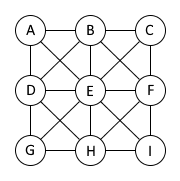
\includegraphics[width=0.24\textwidth]{figures/path/graph_grid}
        \label{sub:grid}
    }
    \subfloat[Circular Graph]{
        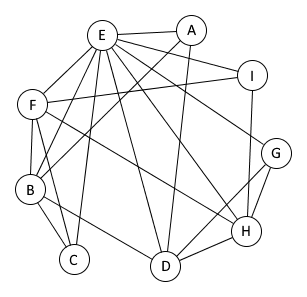
\includegraphics[width=0.24\textwidth]{figures/path/graph_circular}
    }
    \subfloat[Tree Graph]{
    	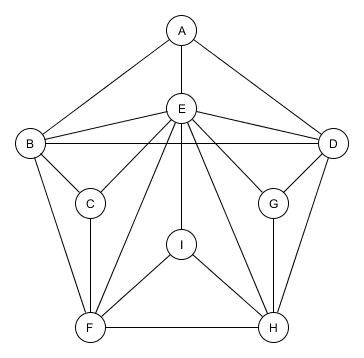
\includegraphics[width=0.24\textwidth]{figures/path/graph_tree}
    }
  	\subfloat[Unstructured Graph]{
  		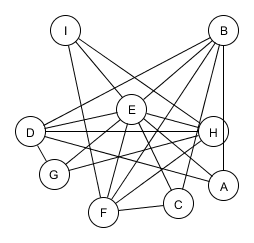
\includegraphics[width=0.24\textwidth]{figures/path/graph_unstructured}
	}
  	\caption{Different Representations of the same Graph}
  	\label{fig:graphs}
\end{figure}

Such a graph can be represented in any way,
as long as none of the described characteristics change.
Figure \ref{fig:graphs} shows four equivalent representations of the same graph.
We chose to omit any numbers for simplicity.

Since our prototype is running on a grid-like map,
the graph shown in Figure \ref{sub:grid} is our preferred representation,
since it is the easiest to relate to the real world for a human.
For the algorithm however, it doesn't matter.
\\\\
\section{Brute-Force}\label{sec:brute}
Brute-force is generally an algorithm,
that only relies on computational power,
instead of clever design.
For path-finding that would mean looking at all possible paths,
and evaluating which one is the shortest.
Brute-force algorithms can be implemented as a depth first search (DFS), or breadth first search (BFS).

\section{Flood Fill}\label{sec:fill}
Flood fill is looking at all neighbour \emph{nodes} from the start,
and looking at all their neighbours.
This process then gets repeated until the finish \emph{node} is reached.
Because the algorithm expands first in breadth,
this is a BFS-algorithm.

The name comes from visualising the algorithm,
which looks fairly similar to a liquid being spilled on a map.
%flood fill can be seen in Figure something later
\cite{Jaimini2017}

\section{Dijkstra}\label{sec:dijkstra}
Dijkstra's algorithm is a small improvement on the flood-fill algorithm explained earlier.
It takes into account the \emph{distances} between two \emph{nodes},
when deciding which \emph{node} to look at next.
Thus prioritising the easier to reach \emph{nodes}, when going to the next iteration.

This is done by storing all \emph{nodes} in a priority queue,
where they are sorted by their \emph{cost to reach}, in ascending order.

The \emph{cost to reach} gets calculated iteratively,
by adding the \emph{cost to reach} of the current \emph{node} together with \emph{distance} to its neighbour.
If that value is smaller than the \emph{cost to reach} currently stored in that neighbour,
the old value gets overwritten.
This process is shown stepwise in Figures \ref{sub:dijk1} through \ref{sub:dijk5}.
Those figures are also available in Appendix \ref{app:path}.\\
Observe how the value for the finish \emph{node} changes in almost every step,
until the finish \emph{node} is the current \emph{node}.

Every time the algorithm needs a new \emph{node} to evaluate its neighbours,
it takes the first element from that list. \cite{Pound2017}

\begin{figure}[h!]
	\begin{center}
		\foreach \dijk in {1,2,3,4,5}
		{
			\subfloat[\dijk. Step]{
				\includegraphics[width=0.175\textwidth]{figures/path/dijk_\dijk.pdf}
				\label{sub:dijk\dijk}
			}
		}
		\caption{Dijkstra's algorithm on a simple map}
		\label{fig:dijksteps}
	\end{center}
\end{figure}
% puts the table closer to the figure
\vspace{-0.75cm}
\begin{table}[h!]
\caption{Colour guide for Figure \ref{fig:dijksteps}}
\centering
\begin{tabular}{|l|p{4cm}|p{4cm}|}
	\hline%-------------------------------------------------------
	\multirow{2}{*}{Colour}	& \multicolumn{2}{c|}{Function}		\\
		 	& Nodes					&Edges						\\
	\hline%-------------------------------------------------------
	Red		&						&Used in current evaluation	\\
	\hline%-------------------------------------------------------
	Orange 	& Current Node			&							\\
	\hline%-------------------------------------------------------
	Green	& Evaluated Neighbour	&							\\
	\hline%-------------------------------------------------------
	White	& Not active yet		&							\\
	\hline%-------------------------------------------------------
	Black  &Shortest Path already found&Not used in current step\\
	\hline%-------------------------------------------------------
\end{tabular}
\end{table}

This approach has a huge benefit for maps,
where \emph{distances} between \emph{nodes} vary widely.
In our case \emph{distances} are one of two possibilities, either $1$ or $ \sqrt{2} $.
Thus making this effectively one implementation of a flood-fill search,
with the benefit, that only one addition needs to be done to implement A*,
which gets explained in Section \ref{sec:astar}.

\section{A*}\label{sec:astar}
A* uses Dijkstra's algorithm as a baseline,
but adds one more step in calculating.
Just like in Dijkstra, the \emph{cost to reach} gets calculated iteratively,
with the same iteration method.
But in A* there is also another value added to that sum,
this value is often called \emph{heuristic}.
It is used to point the algorithm towards the finish node,
and is often the \emph{Euclidean Distance} distance from each node to the finish.
\cite{PoundStar}
The \emph{Euclidean Distance},
is the distance as the crow flies.
It can be calculated with help of the Pythagorean Theorem:
\begin{example}{Pythagorean Theorem used for Euclidean Distance}
  \label{ex:pyth_eucl}
  \begin{equation}
	\sqrt{|A_{X}-B_{X}|^{2}+|A_{Y}-B_{Y}|^{2}}
  \end{equation}
\end{example}


\section{Pathfinding on a grid}
Pathfinding on a grid is slightly different to pathfinding on a regular map,
because all \emph{nodes} tend to have the same amount of neighbours,
and all \emph{edges} have the same or similar \emph{distances}.

In our case \emph{distances} vary between $1$ and $\sqrt{2}$,
the former in the case of vertical or horizontal movement,
the latter for diagonal movement.
Figure \ref{fig:graph_cost} shows the similarities between connections on a grid-based graph.
because of this, the Dijkstra algorithm is losing its major advantage over a simple flood fill.
\begin{figure}[htp]
	\centering
	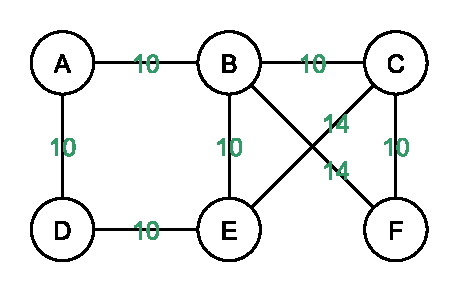
\includegraphics[width=0.5\textwidth]{figures/path/graph_values.pdf}
	\caption{Graph with Labelled Edges}
	\label{fig:graph_cost}
\end{figure}

On a grid, it makes little sense to use the \emph{euclidean distance}.
Because movement is very restricted,
and can only be a multiple of the possible \emph{distances}.
Here it could make more sense to use the \emph{Manhattan Distance},
because that actually represents the minimal possible path.
The \emph{Manhattan Distance} is obtained by the formula shown in Example \ref{ex:manhattan}.
\begin{example}{Manhattan Distance}
  \label{ex:manhattan}
  \begin{equation}
	|X_{A}-X_{B}|+|Y_{A}-Y_{B}|
  \end{equation}
\end{example}


\section{Our implementation}\label{sec:path_implement}
Our explanation of the implementation relies heavily on our program written in C.
Every function explained in this section can also be read in Appendix \ref{app:path}.

Since our map consists of \emph{nodes} with up to eight neighbours,
as explained in Chapter \ref{ch:map}, \todo{does Troels explain this?}
we decided to store this information in a single byte per \emph{node}.
In this byte, the \emph{Least Significant Nibble (LSN)} represents the straight directions N,E,S,W.
The \emph{Most Significant Nibble (MSN)} represents the diagonal directions NE,SE,SW,NW.
Some example bytes can be seen in Table \ref{tab:wallbyte}.

\begin{table}[h!]
\caption{Examples of Bytes representing Walls}
\begin{center}
	\begin{tabular}{|*{8}{m{1cm}|}|l|}
		\hline%-------------------------------
		NE& SE& SW& NW& N & E & S & W & byte\\
		\hline%-------------------------------
		path & path & path & path & path & path & path & WALL & 0x01\\
		path & path & path & path & path & path & WALL & path & 0x02\\
		path & path & path & path & path & path & WALL & WALL & 0x03\\
		path & path & path & path & WALL & WALL & WALL & path & 0x0E\\
		\hline%-------------------------------
		path & path & path & WALL & path & path & path & path & 0x10\\
		path & path & WALL & path & path & path & path & path & 0x20\\
		path & WALL & path & path & path & path & WALL & path & 0x42\\
		WALL & WALL & WALL & WALL & WALL & WALL & WALL & WALL & 0xFF\\
		\hline%-------------------------------
	\end{tabular}
\end{center}
\label{tab:wallbyte}
\end{table}

Listing \ref{lst:defsHBytes} shows how we define the different directions in our program.

\lstinputlisting
[firstline=12,			%starts reading the file from line 12
firstnumber=12,			%starts counting the lines in pdf from 12
lastline=20,			%stops reading the file at line 20
label=lst:defsHBytes,	%label
caption={Definition of Directions in {\tt defs.h}}
]{code/defs.h}
%
After reading the map from the input file,
as explained in Section \ref{sec:map_implement}, \todo{does Troels describe this in ch:map?}
all \emph{nodes} have to be set up for the pathfinding algorithm.
We do this in the function {\tt path\_set\_neighbors}.
Every \emph{node} gets linked to its neighbours by comparing the {\tt walls} value
with the defined directions as shown in Listing \ref{lst:linking}.
Every direction that does not have a wall,
gets linked as a pointer.
If it has a wall, the pointer is set to {\tt NULL}.
We only show the linking of the straight neighbours,
because the diagonal neighbours work basically the same.

\lstinputlisting
[firstline=9,			%starts reading the file from line 9
firstnumber=9,
lastline=20,			%stops reading the file at line 20
label=lst:linking,	%label
caption={Linking of straight Neighbours in {\tt path.c}}
]{code/path.c}
%
The same function also initially sets the {\tt movecost}
(\emph{cost to reach}) to 4095 ({\tt 0xFFF}) for all \emph{nodes},
except for the starting \emph{node},
and lets {\tt parent} point to {\tt NULL}.
This can be seen in Listing \ref{lst:movecost}.

\lstinputlisting
[firstline=35,			%starts reading the file from line 35
firstnumber=35,
lastline=41,			%stops reading the file at line 41
label=lst:movecost,	%label
caption={Setting {\tt movecost} and {\tt parent} in {\tt path.c}}
]{code/path.c}
%
After everything is set up,
the path-finding algorithm can start.

We implemented Dijkstra's algorithm in the function {\tt path\_calculate},
shown in Listing \ref{lst:path}.
Here we have two integers {\tt curx} and {\tt cury} to keep track of the position
and a {\tt currNode} as our current \emph{node}.
The algorithm loops through all \emph{nodes},
until it reaches the finish \emph{node}.
We implemented this as a {\tt while} loop.

To prevent the algorithm from looping infinitely,
in case of a subtle error,
we increment a counter {\tt deadcount} on every iteration
and check whether it surpasses the amount of \emph{nodes}.

Inside the loop we check for every \emph{neighbour},
whether a pointer to it exists
and whether its \emph{cost to reach} is higher than it would be from the current \emph{node}.
In the case that both statements are true,
we update \todo{overwrite?} the neighbours \emph{cost to reach}
and \emph{parent}.

We also remove the current \emph{node} as a neighbour,
because we know the path back and forth cannot be shorter.
This removes one lookup going through three pointers and involving one addition.

\lstinputlisting
[firstline=64,			%starts reading the file from line 64
firstnumber=64,
lastline=88,			%stops reading the file at line 88
label=lst:path,	%label
caption={Calculating the Path in {\tt path.c}}
]{code/path.c}
%
After looking through all neighbours of a \emph{node},
it can be pushed onto the {\tt checked} stack.
And the next node has to be popped from the {\tt unchecked} queue,
before looping to the start of the {\tt while} again.
This can be seen in Listing \ref{lst:node_calc}.

\lstinputlisting
[firstline=127,			%starts reading the file from here
firstnumber=127,
lastline=131,			%stops reading the file at this line
label=lst:node_calc,	%label
caption={Pushing and Popping Nodes in {\tt path.c}}
]{code/path.c}
%
When all \emph{nodes} leading to the finish \emph{node} have been checked,
the full path is in the {\tt checked} stack.
But also every other \emph{node} with a smaller \emph{cost to reach}.
The top element on the stack is also the finish \emph{node},
so the first movement gets described in the bottom of the stack.

This means it is necessary to sort through the stack,
and to only keep the necessary \emph{nodes}.
While doing this we can immediately calculate the movements to be done
and put them on a new stack.
Since the \emph{node}-stack had the finish \emph{node} at the top,
the movement stack will have the finish movement at the bottom.

We calculate the movements out of the coordinates of the \emph{nodes},
in function {\tt path\_calculate\_movement} as can be seen in listing \ref{lst:move_calc}.
Movement can be seen as a vector,
where a change in X coordinate shows movement along the North-South axis,
and change in Y coordinate shows movement along the East-West axis.
If only one axis changes, the resulting movement is straight,
if change happens on both axes, it is diagonal.

\lstinputlisting
[firstline=145,			%starts reading the file from line 64
firstnumber=145,
label=lst:move_calc,	%label
caption={Pushing and Popping Nodes in {\tt path.c}}
]{code/path.c}
%
